\documentclass[class=report,crop=false, 12pt]{standalone}
\usepackage[screen]{../scratch}

\begin{document}


\titre[E]{Si ... alors ...}
%===============================


\begin{enigme}
\sauteligne

\begin{itemize}
  \item Scratch part de $x=-200$, $y=0$.
  \item Scratch s'oriente à $80$\textdegree\ (par rapport au Nord).
  \item Ensuite, on répète indéfiniment :
    \begin{itemize}
      \item avancer de 5,
      \item si $x > y$, alors on affiche $x$.
    \end{itemize}
\end{itemize}

\bigskip

\textbf{Question.} Quelle est la première valeur de $x$ affichée ?
(On arrondira $x$ à l'entier supérieur ou inférieur.)


%\begin{solution}
%$x=46,20$ donc la réponse est $46$ ou $47$.
%\end{solution}

\end{enigme}


\begin{enigme}


Scratch se déplace en fonction des touches de flèches pressées.
Il part de $x=0$, $y=0$ et est orienté vers la droite.

\begin{itemize}
  \item Si la flèche droite ($\rightarrow$) est pressée, alors Scratch avance de $30$
  (et attend $0.2$ seconde).
  \item Si la flèche haut ($\uparrow$) est pressée, alors Scratch tourne de $15$\textdegree\  vers la gauche (et attend $0.2$ seconde).  
\end{itemize}

Programme Scratch afin qu'il suive ces consignes.

\bigskip

Voici la séquence d'instructions saisie par un élève :

{\Large
$$\rightarrow \quad \rightarrow \quad \uparrow \quad \rightarrow \quad \uparrow \quad \rightarrow \quad \uparrow \quad \uparrow \quad \rightarrow \quad 
\rightarrow \quad \rightarrow \quad \uparrow \quad \rightarrow $$
}

\bigskip

\textbf{Question.} Quelle est la valeur de l'abscisse $x$ à la fin de ces instructions ?
(On arrondira la réponse à l'entier supérieur ou inférieur.)

%\begin{solution}
%$x=167,72$ donc la réponse est $167$ ou $168$.
%\end{solution}

\end{enigme}



\begin{enigme}

Scratch avance si certaines conditions sont validées.

\medskip

\begin{minipage}{0.49\textwidth}
\begin{itemize}
  \item Si \og{}$2<3$\fg{}, alors Scratch avance de $30$.
  
\vspace*{6ex}  
  
  \item Si \og{}$2+3=4$\fg{}, alors Scratch avance de $40$.
  
\vspace*{6ex}    
  
  \item Si \og{}$2 \times 3 > 7$ \textbf{ou} $9-5 > 3$\fg{}, alors Scratch avance de $50$. 
  
\vspace*{6ex}    
     
  \item Si \og{}\textbf{non} ($3 \times 4 = 12$)\fg{}, alors Scratch avance de $60$. 
\end{itemize}   
\end{minipage}
\begin{minipage}{0.49\textwidth}
\begin{center}
  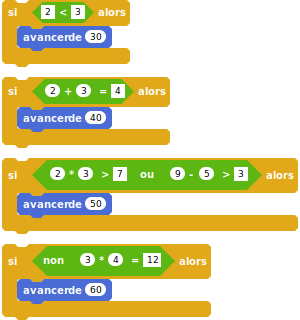
\includegraphics[scale=\scalebloc,scale=0.8]{code-04-eg3}
\end{center}
\end{minipage}

%\medskip
%Quelles sont les conditions qui seront vérifiées ? Vérifie en programmant Scratch.

\bigskip

\textbf{Question.} Au total, après toutes ces instructions, de combien de pas Scratch a-t-il avancé ?


%\begin{solution}
%Les assertions 1 et 3 sont vraies, donc Scratch avance de $30+50=80$.
%\end{solution}

\end{enigme}


\end{document}

